\documentclass[xcolor=dvipsnames,12pt]{beamer}
\definecolor{UBCblue}{rgb}{0.04706, 0.13725, 0.26667} % UBC Blue (primary)

\usecolortheme[named=UBCblue]{structure}
\usefonttheme[onlymath]{serif}
\usetheme{Boadilla}
\usepackage{graphicx}
\usepackage{float} 
\usepackage{subfigure}
\usepackage{caption}
\usepackage{amsmath}
\usepackage{mathtools}
\DeclarePairedDelimiter\floor{\lfloor}{\rfloor}
\usepackage{comment}
\usepackage{makecell}
\usepackage{color}
\usepackage{fbox} 
\usepackage[table]{xcolor}
\input{Symbol_Shortcut.tex}
\setbeamertemplate{caption}[numbered]
\setbeamertemplate{bibliography item}{\insertbiblabel}

\usepackage[font={scriptsize}]{caption} % set caption font size to be scriptsize
\usepackage[absolute,overlay]{textpos}  % for some textbox
\usepackage{tikz}
\usetikzlibrary{calc}
\usepackage{multirow} % for multirow in table
\usepackage{appendix}
\usepackage{hyperref} % for hyperlink to appendix

\title[]{Natthakrit Toemphinijtham}
\date{13 October 2026}

\AtBeginSection[]
{
\begin{frame}<beamer>
	\frametitle{Outline}
	\tableofcontents[currentsection]
\end{frame}
}

\newcommand{\myfootercenter}{ITRI Communication Protocol Development Engineer (M201)}
\newcommand{\setfooter}[1]{\renewcommand{\myfootercenter}{#1}}

\setbeamertemplate{footline}
{%
  \leavevmode%
  \hbox{%
    \begin{beamercolorbox}[wd=.25\paperwidth,ht=2.5ex,dp=1ex,left]{author in head/foot}%
      \hspace{2ex} Natthakrit Toemphinijtham
    \end{beamercolorbox}%

    \begin{beamercolorbox}[wd=.6\paperwidth,ht=2.5ex,dp=1ex,center]{title in head/foot}%
        \myfootercenter  % This now uses your custom variable
    \end{beamercolorbox}%

    \begin{beamercolorbox}[wd=.15\paperwidth,ht=2.5ex,dp=1ex,right]{date in head/foot}%
    %   \insertshortdate \hspace{2ex}
      \insertframenumber/\inserttotalframenumber
      \hspace{2ex}
    \end{beamercolorbox}%
  }%
  \vskip0pt%
}
%%%%%%%%%%%%%%%%%%%%%%%%%%%%%%%%%%%%%%%%%%%%%%%%%%%%%%%%%%%%%%%%%%%%%%%%%%%%%%%%%%%%%%%%%%%%%%%%%%%%%%%
%%%%%%%%%%%%%%%%%%%%%%%%%%%%%%%%%%%%%%%%%%%%%%%%%%%%%%%%%%%%%%%%%%%%%%%%%%%%%%%%%%%%%%%%%%%%%%%%%%%%%%%
\begin{document}
%=================================================================
\setfooter{5G NR PHY Transceiver}
\begin{frame}

    \vspace{1.5cm}
    
    \begin{center}
    
        {\Large \textbf{5G NR PHY Transceiver}} \\[1.3cm]

        \begin{scriptsize}
            \textbf{GitHub repository}: \url{https://github.com/ryuvidd/NR_Communication_Pipeline.git} \\
            \textbf{reference}: 3GPP TS 38.211-38.214 \\
            \textbf{keywords}: OFDM, Channel Estimation, Channel Coding, Equalization\\[0.8cm]    
        \end{scriptsize}
        
        Developed by \\
        \textbf{Natthakrit Toemphinijtham} \\[0.8cm]
        October 13, 2026
    
    \end{center}
    \end{frame}

%=================================================================
\setfooter{System Architecture}
\begin{frame}{System Architecture}
\begin{small}  
    \begin{figure}
        \centering
        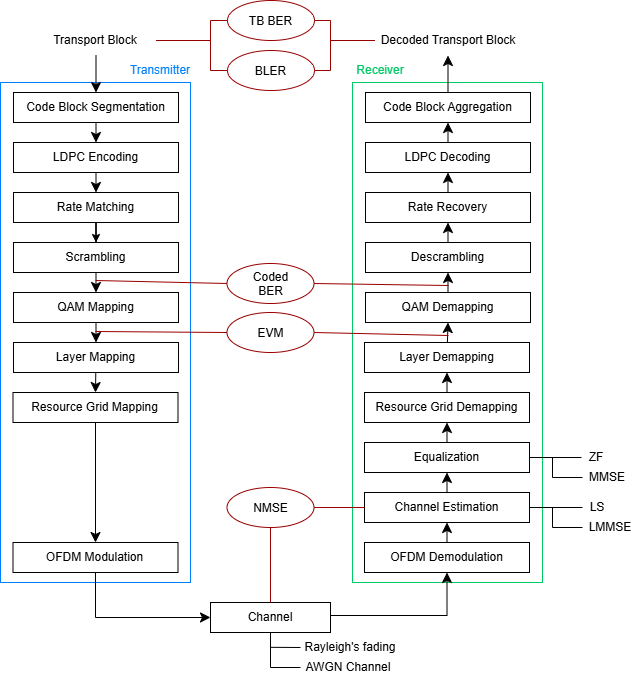
\includegraphics[width=0.61\textwidth]{figs/system_architecture.png} 
        % \caption{Transceiver pipeline.}
    \end{figure}
\end{small}
\end{frame}

%=================================================================
\setfooter{System Configurations}
\begin{frame}{System Configurations}
\begin{footnotesize}
    \begin{table}[t]
        \tiny
        \centering
        \caption{System configuration.}
        \label{Table_system_config}
    
        \begin{tabular}{|p{4cm}|>{\centering\arraybackslash}p{2cm}|}
            \hline
            \rowcolor{gray!15}
            \multicolumn{2}{|l|}{\textbf{Carrier and Bandwidth Part Configuration}} \\
            \hline
            Carrier frequency & 2.5 GHz \\
            Subcarrier spacing & 30 kHz \\
            Number of OFDM symbols per slot & 14 \\
            Number of allocated PRBs & 50 \\
            Allocated PRBs & $5 \sim 14$ \\
            \hline
            \hline

            \rowcolor{gray!15}
            \multicolumn{2}{|l|}{\textbf{PDSCH Configuration}} \\
            \hline
            Allocated OFDM symbols & $2 \sim 13$ \\
            Modulation order, $Q_m$ & 4 \\
            Coding rate, $R$ & 0.3 \\
            Number of transmission layers & 1 \\
            \hline
            \hline

            \rowcolor{gray!15}    
            \multicolumn{2}{|l|}{\textbf{DMRS Configuration}} \\
            \hline
            DMRS configuration type & Type 1 \\
            DMRS length & single-symbol \\ 
            Mapping type & Type A \\
            First DMRS OFDM symbol & 2 \\
            Additional DMRS positions & None \\
            \hline
            \hline

            \rowcolor{gray!15}    
            \multicolumn{2}{|l|}{\textbf{Channel Configuration}} \\
            \hline
            Model & Rayleigh fading \\
            Velocity & 15 m/s \\
            Delays & $\{0,100,300\}$ ns \\
            \hline
            \hline

            \rowcolor{gray!15}    
            \multicolumn{2}{|l|}{\textbf{Receiver Configuration}} \\
            \hline
            Channel estimator & LS, LMMSE \\
            Equalizer & ZF, MMSE \\
            LDPC max iterations & 10 \\
            \hline
    
        \end{tabular}
    \end{table}

\end{footnotesize}
\end{frame}

%=================================================================
\begin{frame}{Resource Grid per PRB}
\begin{small}  
    \begin{figure}
        \centering
        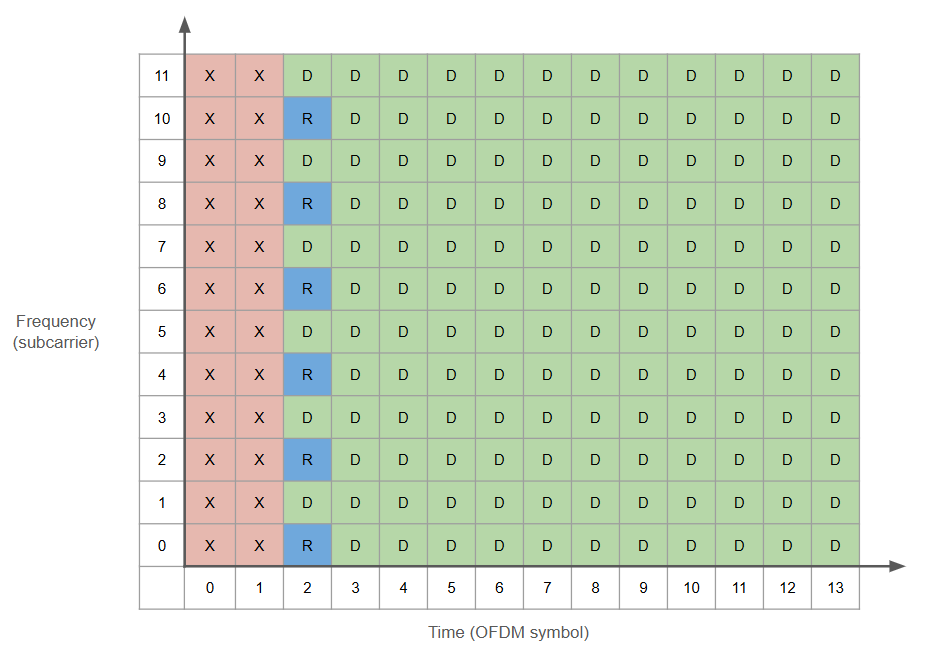
\includegraphics[width=0.7\textwidth]{figs/ResourceGrid.png} 
    \end{figure}

    \begin{figure}
        \centering
        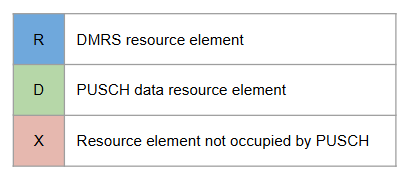
\includegraphics[width=0.3\textwidth]{figs/RG_notation.png} 
    \end{figure}
\end{small}
\end{frame}

%=================================================================
\setfooter{System Model}
\begin{frame}{System Model}
\begin{footnotesize}
    Let $N_R$, $N_T$, and $N_L$ be number of antennas at the receiver, transmitter, and number of transmission layer, respectively.  Each received resource element $(k,l)$ is modeled as
    \begin{equation}
        \begin{aligned}
            \mathbf{y}_{k,l} 
            &= \mathbf{H}_{k,l} \mathbf{G}_{k,l} \mathbf{x}_{k,l} + \mathbf{w}_{k,l} \\
            &\triangleq \mathbf{H}_{\rm{eff},k,l} \mathbf{x}_{k,l} + \mathbf{w}_{k,l} \\
            &= (\mathbf{x}_{k,l}^T \otimes \I_{N_R}) \rm{vec}(\mathbf{H}_{\rm{eff},k,l}) + \mathbf{w}_{k,l} \\
            &\triangleq \tbX_{k,l} \mathbf{h}_{\rm{eff},k,l} + \mathbf{w}_{k,l}
        \end{aligned}
        \label{eq:system_model}
    \end{equation}
    where 
    \begin{itemize}
        \footnotesize
        \item $\mathbf{y}_{k,l} \in \complex^{N_R \times 1}$ is the received symbol,
        \item $\mathbf{H}_{k,l} \in \complex^{N_R \times N_T}$ is the channel matrix,
        \item $\mathbf{G}_{k,l} \in \complex^{N_T \times N_L}$ is the precoder matrix,
        \item $\mathbf{H}_{\rm{eff},k,l} \in \complex^{N_R \times N_L} \triangleq \mathbf{H}_{k,l} \mathbf{G}_{k,l}$ is effective channel matrix,
        \item $\mathbf{x}_{k,l} \in \complex^{N_L \times 1}$ is the transmitted symbol,
        \item $\mathbf{w}_{k,l} \in \complex^{N_R \times 1}$ is noise vector.
    \end{itemize}

\end{footnotesize}
\end{frame}

%=================================================================
\setfooter{Algorithmic Comparisons}
\begin{frame}{Algorithmic Comparisons: Channel Estimators}
\begin{footnotesize}
    \begin{itemize}
        \item[1.] \textbf{Least Square (LS) estimator} \\
        Assuming the channel is constant across $M$ DMRS observations, the system model can be written as $\Y = \H_{\rm{eff}} \X + \W$, where $\Y \in \complex^{N_R \times M}$ and $\X \in \complex^{N_L \times M}$.  The LS esitmate is 
        \begin{equation}
            \hbH_{\rm{eff}} = \Y \X^H (\X \X^H)^{-1}
        \end{equation}
        assuming $\X^H \X$ is invertible.  The channel estimates at data resource elements are obtained through interpolation in frequency and time.

        For SISO system, the system model is reduced to $y_{k,l} = h_{k,l} x_{k,l} + w_{k,l}$, which makes LS estimates become element-wise division,
        \begin{equation}
            \hat{h}_{k,l} = \frac{y_{k,l}}{x_{k,l}}.
        \end{equation}
    \end{itemize}

\end{footnotesize}
\end{frame}

%=================================================================
\begin{frame}{Algorithmic Comparisons: Channel Estimators}
\begin{footnotesize}
    \begin{itemize}
        \item[2.] \textbf{Linear Minimum Mean-Squared Error (LMMSE) Estimator} \\

        Let $M$ and $K$ denote the number of DMRS resource elements in the $l$th OFDM symbol and the number of allocated subcarriers, respectively. The received DMRS observations are modeled as
        \begin{equation}
            \mathbf{y} = \mathbf{A}\mathbf{h} + \mathbf{w},
        \end{equation}
        where $\mathbf{y} \in \mathbb{C}^{M N_R \times 1}$ and $\mathbf{h} \in \mathbb{C}^{K N_R N_L \times 1}$ is the vectorized effective channel over the $K$ allocated subcarriers.  The block-sparse observation matrix $\A \in \complex^{M N_R \times K N_R N_L}$ contains nonzero blocks $\mathbf{x}_m^T \otimes \mathbf{I}_{N_R}$, corresponding to the known pilot vector $\mathbf{x}_m$ at each DMRS resource element.

        The LMMSE channel estimate is given by
        \begin{equation}
        \hbh_{\rm{LMMSE}} = \bmu_h + \R_{hh} \A^H \left( \A \R_{hh} \A^H + \sigma_n^2 \I_{M N_R} \right)^{-1} \left( \y - \A \bmu_h \right),
        \end{equation}
        where $\bmu_h$ and $\R_{hh}$ denote the channel mean vector and channel covariance matrix, respectively, and $\sigma_n^2$ is the noise variance.
    \end{itemize}

\end{footnotesize}
\end{frame}

%=================================================================
\begin{frame}{Algorithmic Comparisons: Equalizers}
    \begin{footnotesize}
        \begin{itemize}
            \item[1.] \textbf{Zero-Forcing (ZF) Equalizer} \\

            For each resource element $(k,l)$, the received symbol is modeled as
            \begin{equation}
                \y_{k,l} = \hbH_{\rm{eff},k,l} \x_{k,l} + \w_{k,l},
            \end{equation}
            where $\hbH_{\rm{eff},k,l}$ denotes the estimated effective channel matrix.  The ZF equalizer estimates the transmitted symbols by computing
            \begin{equation}
                \hat{\x}_{k,l} = (\hbH_{\rm{eff},k,l}^H \hbH_{\rm{eff},k,l})^{-1} \hbH_{\rm{eff},k,l}^H \y_{k,l}.
            \end{equation}
            
        \end{itemize}
    \end{footnotesize}
\end{frame}

%=================================================================
\begin{frame}{Algorithmic Comparisons: Equalizers}
    \begin{footnotesize}
        \begin{itemize}
            \item[2.] \textbf{Minimum Mean-Squared Error (MMSE) Equalizer} \\

            Assuming independent, zero-mean transmitted symbols with covariance $E_s\mathbf{I}$ and spatially white noise with covariance $\sigma_n^2\mathbf{I}$, the MMSE estimate is
            \begin{equation}
                \hat{\x}_{k,l} = \left( \hbH_{\rm{eff},k,l}^H \hbH_{\rm{eff},k,l} + \frac{\sigma_n^2}{E_s}\mathbf{I}_{N_L} \right)^{-1} \hbH_{\rm{eff},k,l}^H \y_{k,l}.
            \end{equation}
            Unlike ZF, MMSE accounts for the noise variance to balance interference suppression and noise enhancement.  As the noise variance approaches zero, the MMSE equalizer approaches ZF when the channel matrix has full column rank.
        \end{itemize}
    \end{footnotesize}
\end{frame}

%==============================================================
\setfooter{Evaluation Metrics}
\begin{frame}{Evaluation Metrics}
\begin{footnotesize}
    % \scriptsize
    \begin{equation}
        NMSE = \frac{\sum_{m=1}^M \sum_{k \in \mathcal{K}} \sum_{l \in \mathcal{L}} | \hat{H}_{m,k,l} - H_{m,k,l} |^2}{\sum_{m=1}^M \sum_{k \in \mathcal{K}} \sum_{l \in \mathcal{L}} | H_{m,k,l} |^2}
    \end{equation}
    where $\mathcal{K}$ and $\mathcal{L}$ are sets of indices of allocated subcarrier and OFDM symbol locations, respectively.  $M=1000$ is the number of Monte-Carlo experiment.
    
    \begin{equation}
        EVM = \sqrt{\frac{\sum_{m=1}^M \sum_{i=1}^N | \hat{X}_{i} - X_{i} |^2}{\sum_{m=1}^M \sum_{i=1}^N | X_{i} |^2}},
    \end{equation}
    where $N$ is the number of QAM symbols and $X_i$ is the complex symbol at $i$th index.

    \begin{equation}
        BER = \frac{1}{M} \sum_{m=1}^{M} \frac{\text{total error bits of $m$ th experiment}}{\text{total transmitted bits}}
    \end{equation}
    
    \begin{equation}
        BLER = \frac{1}{M} \sum_{m=1}^{M} \frac{\text{number of erroneous blocks}}{\text{total transmitted blocks}}
    \end{equation}    
    
\end{footnotesize}
\end{frame}

%==============================================================
\setfooter{Simulation Results}
\begin{frame}{\begin{large}Simulation Results: Channel Estimation Performance\end{large}}
\begin{footnotesize}
    Evaluate an SISO OFDM system over a Rayleigh fading channel, comparing LS and LMMSE channel estimators with a fixed MMSE equalizer at the initial transmission.
    % \begin{column}{0.4\textwidth}
        \begin{figure}
            \centering
            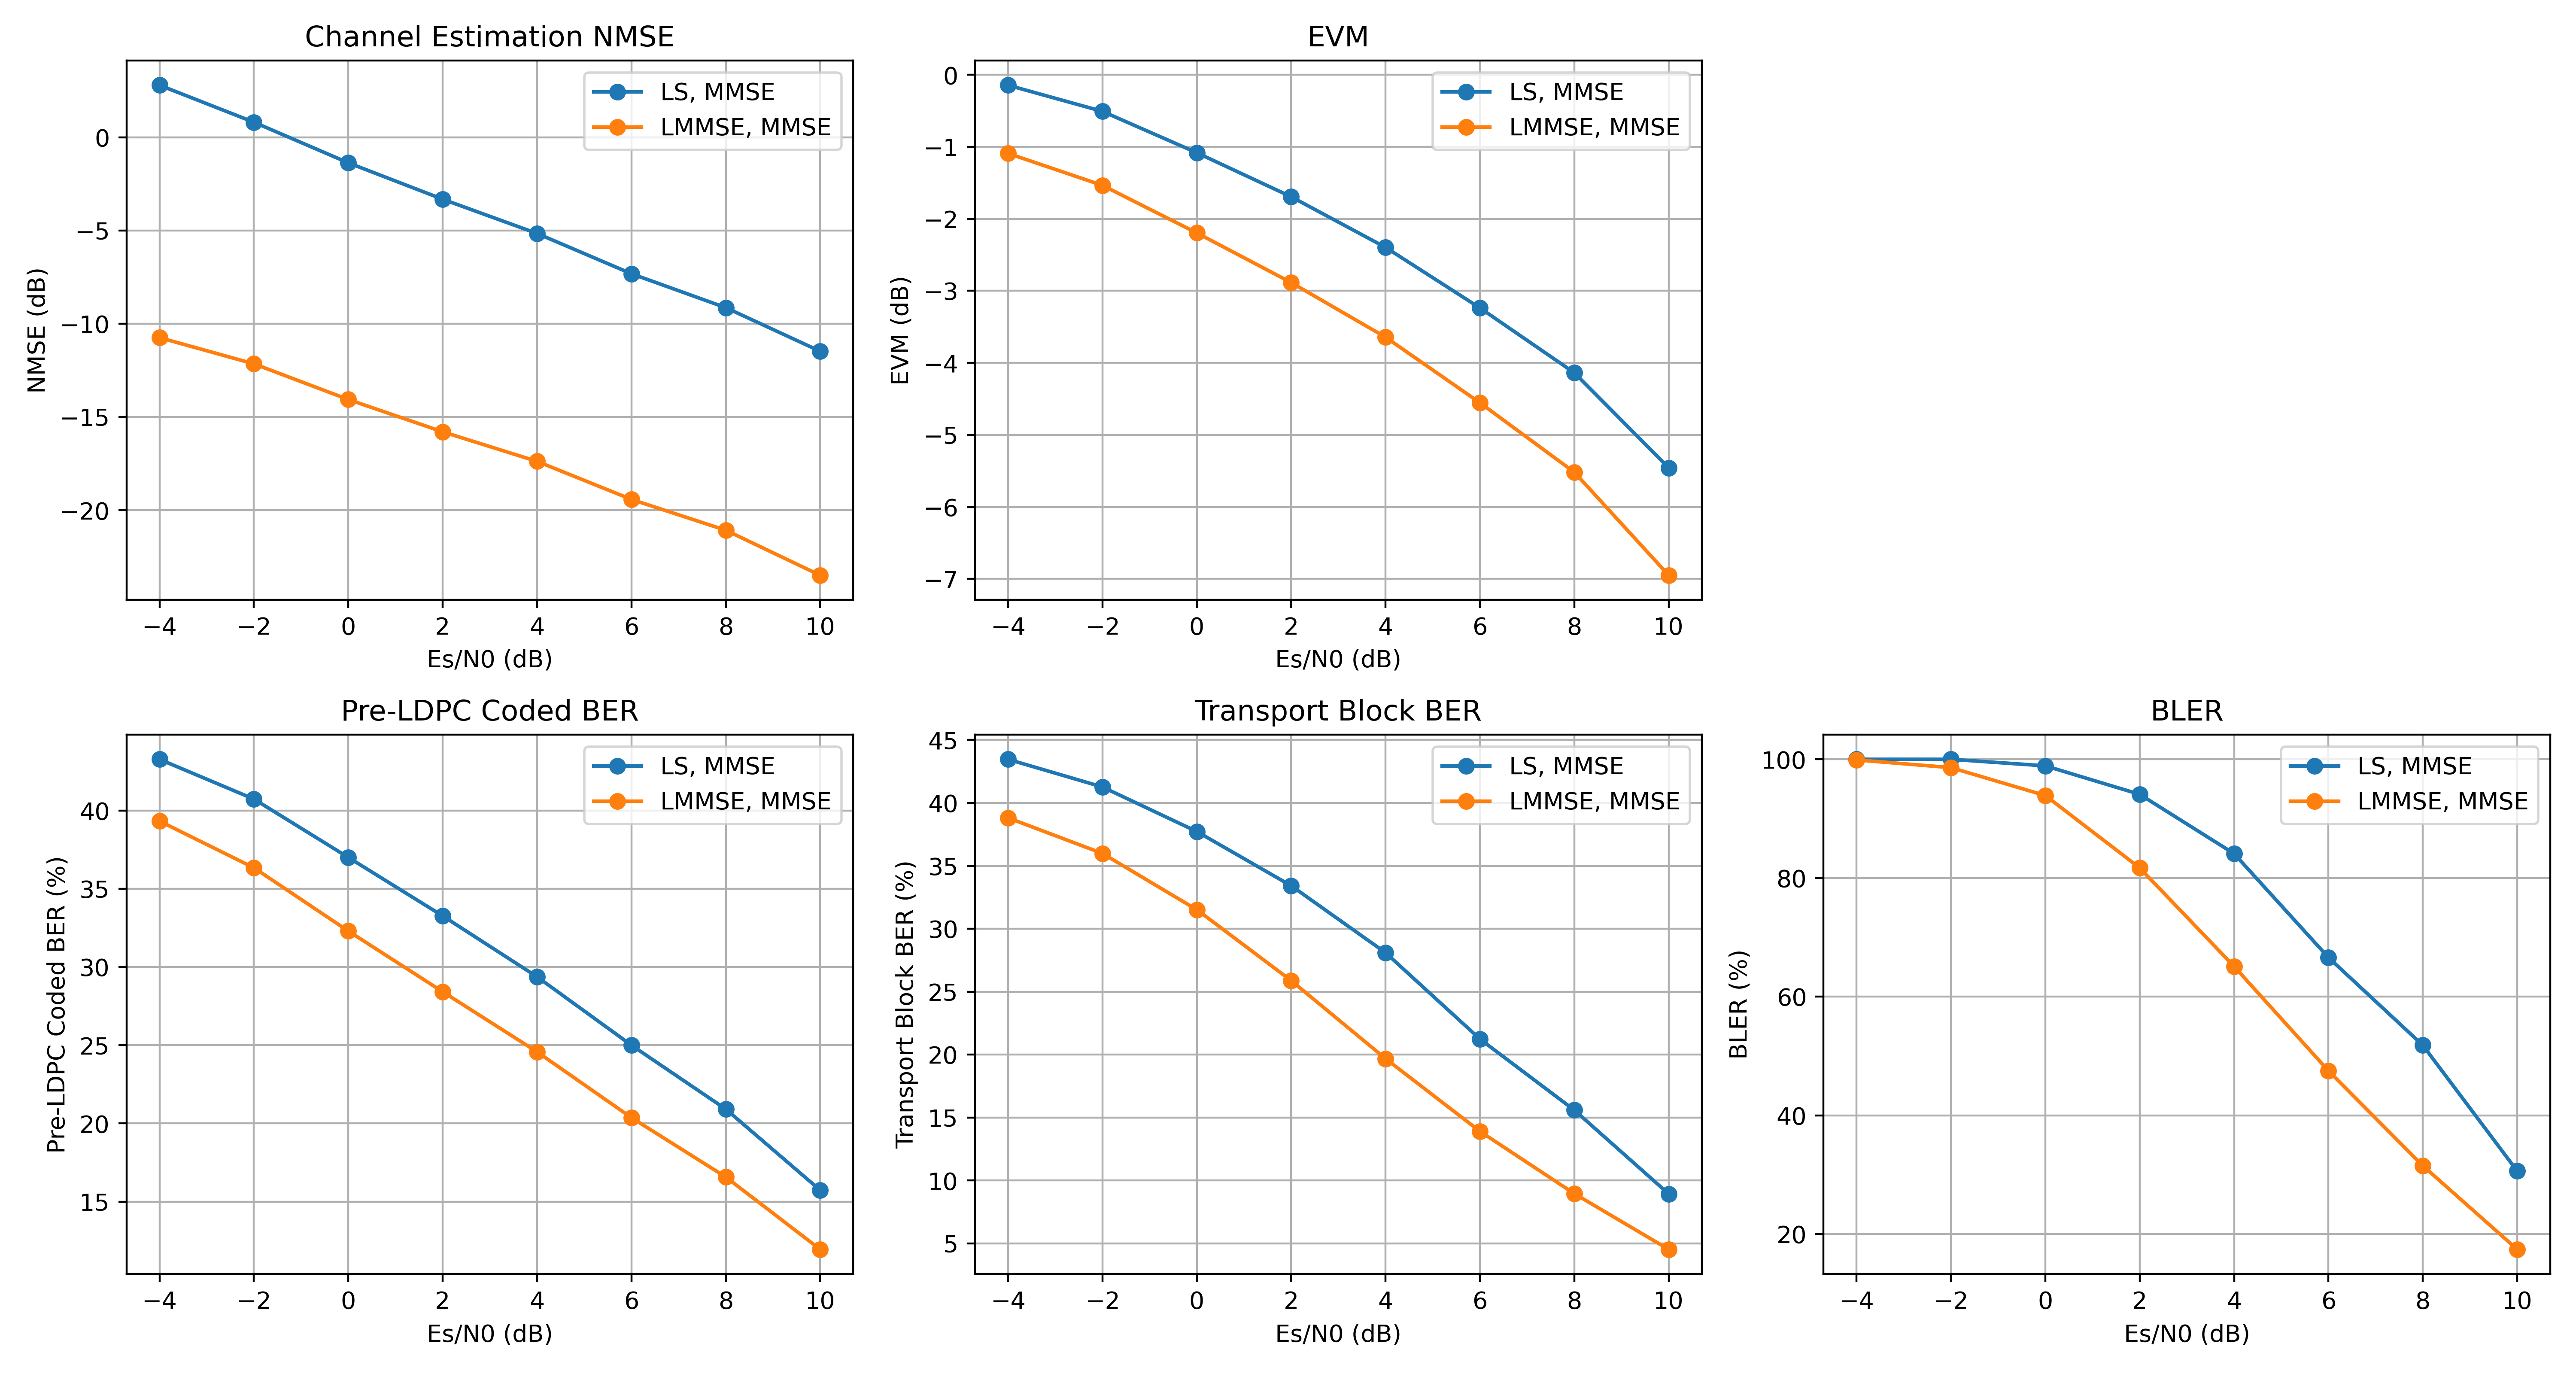
\includegraphics[width=0.9\textwidth]{figs/Results_LS_LMMSE_One_Transmission.png}
        \end{figure}
    % \end{column}
    
\end{footnotesize}
\end{frame}

%==============================================================
\begin{frame}{\begin{large}Simulation Results: HARQ Performance\end{large}}
\begin{footnotesize}
    Evaluate HARQ retransmission performance in an SISO OFDM system over a Rayleigh fading channel, using LMMSE channel estimation and MMSE equalization.
    \begin{figure}
        \centering
        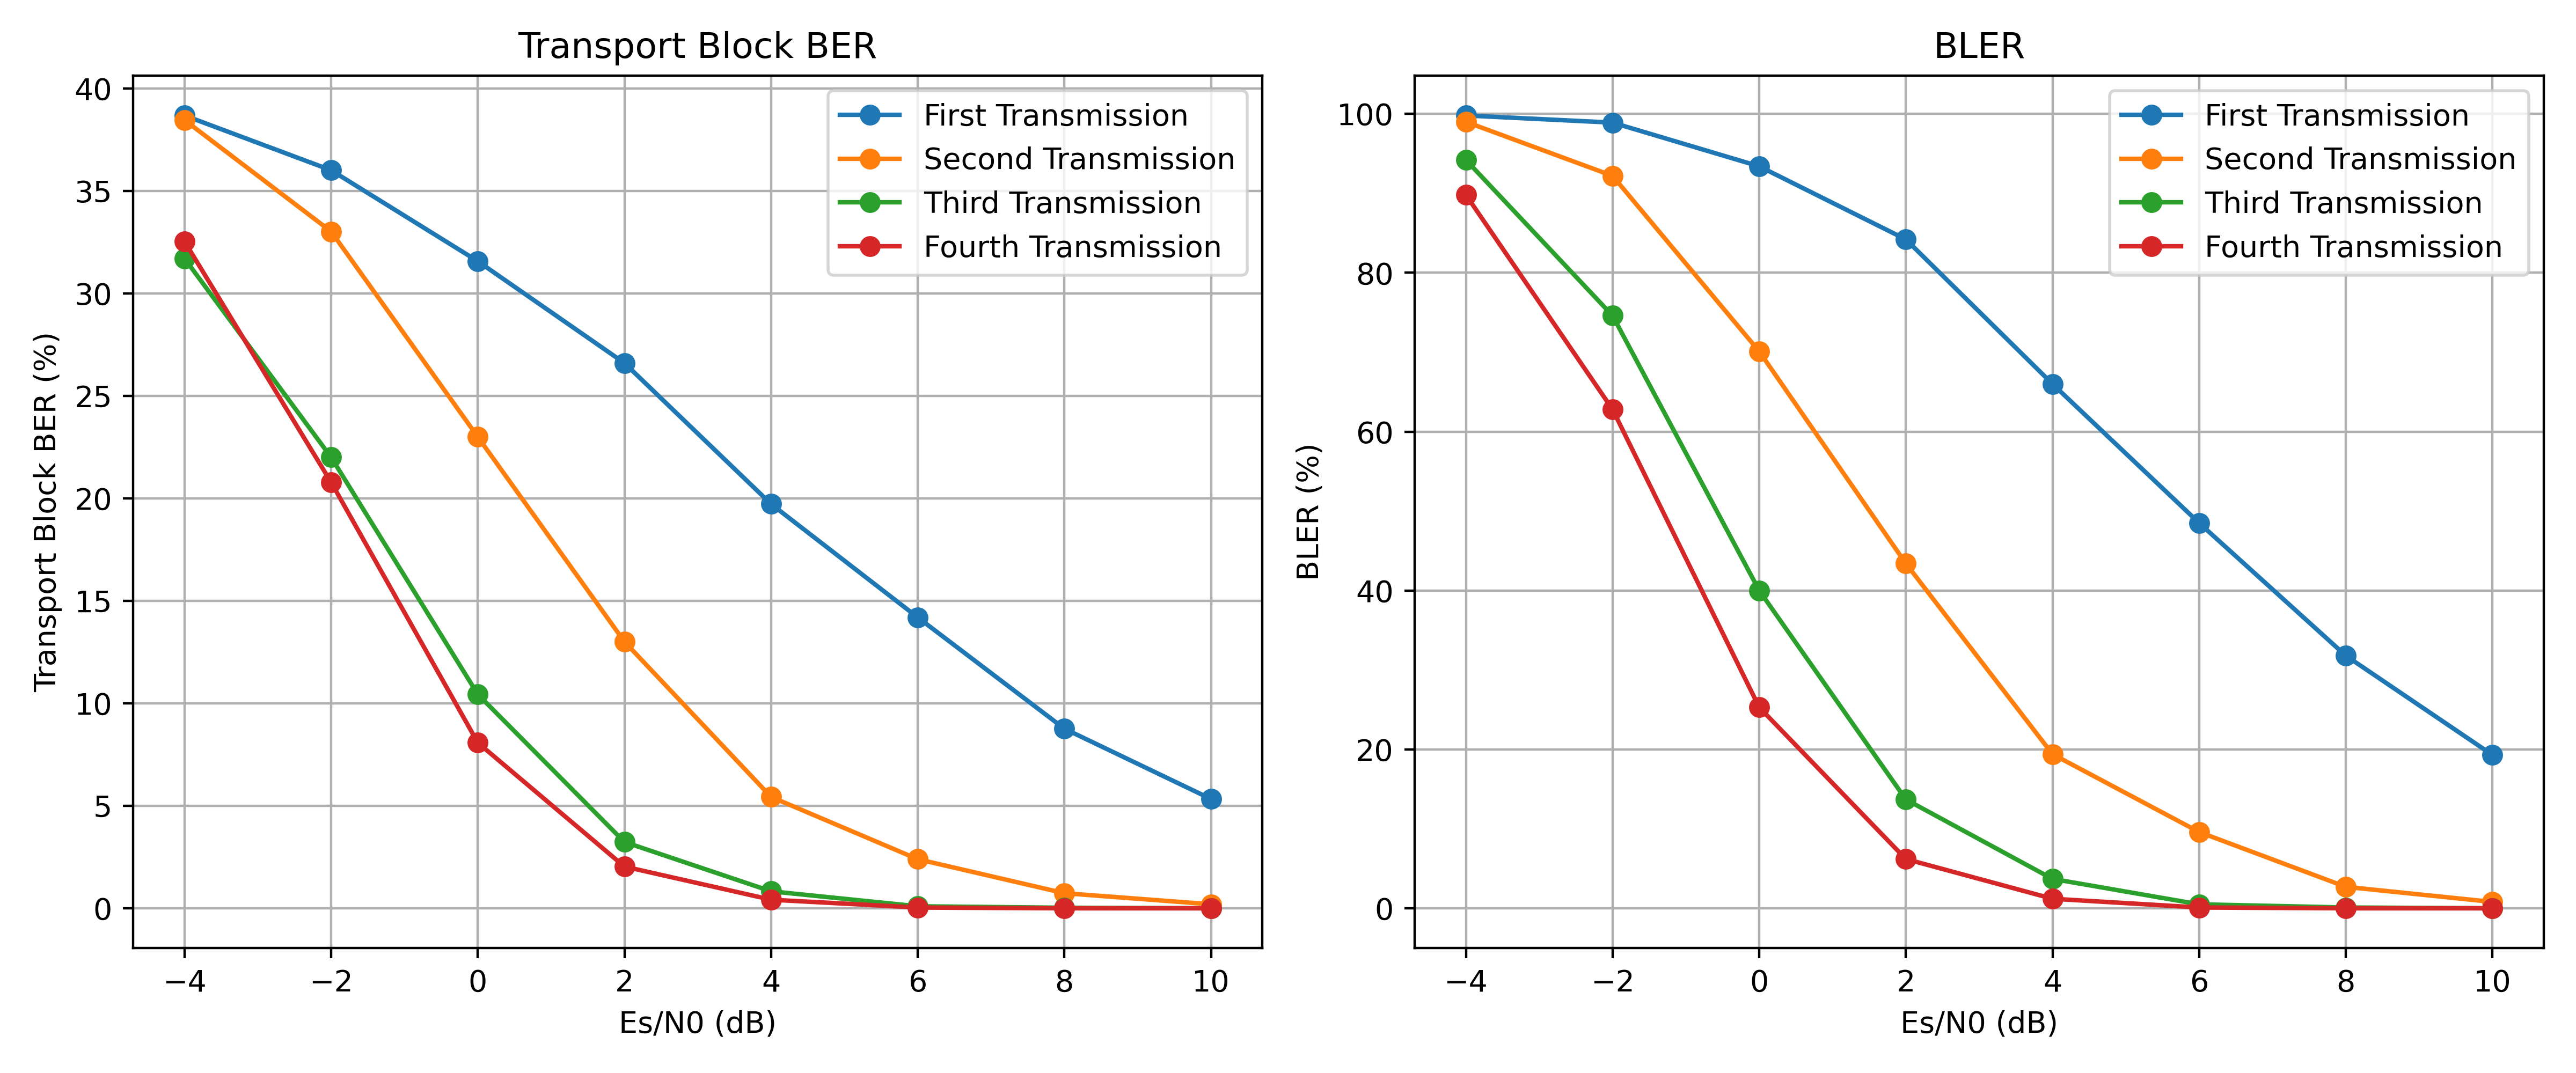
\includegraphics[width=1\textwidth]{figs/Results_LMMSE_MMSE_RVs.png}
    \end{figure}
    
\end{footnotesize}
\end{frame}

%=================================================================
\setfooter{Future Work}
\begin{frame}{Future Work}
\begin{footnotesize}
    \begin{itemize}
        \item[1.] MIMO system implementation
        \begin{itemize}
            \item implement layer mapping and precoding
            \item implement matrix-based ZF and MMSE detection
        \end{itemize}
        \item[2.] Enhance 5G NR configuration processing
        \begin{itemize}
            \item DCI and DMRS configuration parser to derive PDSCH resource allocation and DMRS mapping
        \end{itemize}
        \item[3.] Channel modeling and algorithm optimization
        \begin{itemize}
            \item Support diverse and realistic wireless channel models
            \item Implement and evaluate additional channel estimation and equalization algorithms
        \end{itemize}
    \end{itemize}
    
\end{footnotesize}
\end{frame}

%==============================================================

\end{document}